\chapter{IMPLEMENTATION AND RESULTS}
\label{ch:implementation}

The software engineering effort and measured results are described, including the implementation of the backend and frontend of the software as well as the integration of H5P and the implementation of security controls, followed by performance results for the AI pipeline, API endpoints, scalability, and support for the Vietnamese language.

% ─────────────────────────────────────────────────────────────────────────────
\section{Implement}

\subsection{Backend and Frontend Implementation}

\textbf{User-Centred Design Process and Iterative Prototyping.}

The interface was designed through a three-stage process before any frontend code was written.
\begin{itemize}
    \item \textbf{(1) Conceptual Design:} User flow diagrams were created for the two primary workflows---manual authoring and AI-assisted generation. These flows were reviewed against Nielsen's heuristics to identify sources of extraneous cognitive load before any wireframing began.
    \item \textbf{(2) Wireframing and Heuristic Evaluation:} High-fidelity wireframes were built in Figma and evaluated against three heuristics: visibility of system status (ensuring loading indicators were present during AI generation), error prevention (disabling submit buttons until validation passes), and recognition over recall (displaying the transcript text alongside the video so instructors don't need to memorize dialogue).
    \item \textbf{(3) Prototype Testing:} The interactive Figma prototype was tested with two senior IT students using a think-aloud protocol. This revealed three usability problems: timestamp fields weren't auto-populated when adding a new question; AI-related status messages were too subtle to notice; and button labels on the injection panel were ambiguous. All three were fixed before formal evaluation. The resulting workflow reduced the total number of interface interactions needed to author a three-question interactive video from 47 (in the legacy WordPress baseline) to 8 in the new platform.
\end{itemize}

\textbf{Backend Engineering Architecture.}

The backend runs on Node.js~\cite{nodejs2023} with Express.js~\cite{expressjs2023}, using a standard middleware stack. The \texttt{helmet} middleware configures HTTP security headers. CORS is locked to allowed origins. \texttt{express-rate-limit} protects sensitive routes from brute-force vectors. Winston provides structured JSON logging for observability.

Authentication is stateless using JWT with a 7-day expiry. Passwords are hashed with \texttt{bcryptjs} at cost factor 12. When a video file is uploaded, the backend spawns a child process invoking FFmpeg~\cite{ffmpeg2023} to extract a thumbnail and read the file's metadata (duration, resolution, codec) for validation.

\textbf{Frontend React SPA Architecture.}

The frontend is a React 18 SPA built with Vite~\cite{vite2023} and TypeScript~\cite{typescript2023}. Zustand manages global state---the authenticated user profile, the active video object, and the array of AI suggestions. The component structure is organized around the ``co-location'' principle from cognitive load theory: rather than splitting tasks across pages, the editor presents three vertically scrolling panels side by side. The left panel handles video upload and metadata. The centre panel has the video player and the custom H5P timeline. The right panel shows the AI suggestion review and manual authoring forms.

How the frontend handles the AI generation process is worth explaining in detail. LLM generation can take upwards of 15 seconds, and waiting for a synchronous HTTP response would freeze the UI. The frontend uses the native \texttt{EventSource} API to open an SSE connection with the backend instead. As questions are validated and enriched on the backend, they stream individually to the UI, appearing one at a time rather than all at once. From a user experience perspective, this makes the system feel responsive and active---the instructor can start reviewing the first questions while the rest are still being generated.

Type safety is maintained across the network boundary. The frontend TypeScript interfaces mirror the backend Zod validation schemas, so a \texttt{MultiChoice} suggestion received from the AI has the same type shape as one the instructor creates manually.
\clearpage
\subsection{Security and H5P Integration}

\textbf{Lumieducation H5P Server Library Integration.}

The headless \path{@lumieducation/h5p-server} library~\cite{lumieducation2023} provides four structural advantages as a Node.js service:

\begin{itemize}
  \item \textbf{Automated Library Management.} H5P library ZIP archives and their dependency trees are automatically downloaded from the H5P hub on first use and cached in \texttt{h5p-libraries/}. Library versions are locked per platform version.
  \item \textbf{Decoupled Content CRUD.} H5P content parameters are stored as clean JSON documents in \texttt{h5p-content/}, indexed by UUID.
  \item \textbf{Standards-Compliant Package Export.} The library generates standards-compliant \texttt{.h5p} ZIP archives on demand, bundling the required JavaScript libraries, content JSON, and media assets. These archives are structurally identical to those produced by the official WordPress H5P plugin, ensuring 100\% importability into Moodle, Canvas, and Blackboard.
  \item \textbf{Preview Rendering.} The companion \path{@lumieducation/h5p-express} integration mounts an H5P rendering router at \texttt{/h5p/} that produces the HTML, CSS, and JavaScript bundle needed to embed H5P content in an instructor preview panel. When the preview iframe loads, the browser fetches the \texttt{H5P.InteractiveVideo} JavaScript library from \path{/h5p/libraries/}. This library registers a time-update listener on the video element; when playback reaches a registered timestamp, the library pauses the video and renders the interaction overlay---a question form matching the interaction type (e.g., Multiple Choice, Fill in the Blanks)---directly over the video. The learner submits a response before playback resumes. This same mechanism applies when the exported \texttt{.h5p} package is imported into Moodle or Canvas: the LMS serves the H5P libraries from its own cache but the interaction logic is identical.
\end{itemize}

\textbf{How AI Suggestions Become H5P Interactions: The \texttt{injectAll()} Function.}

When an instructor accepts a set of AI-generated suggestions in the UI, those suggestions are sent as a JSON array to the \texttt{POST}~\path{/api/ai/inject} endpoint. The backend calls \texttt{injectAll()} from \texttt{aiInjectionService.js}:
\clearpage

\begin{lstlisting}[language=JavaScript,caption={injectAll() — key structure: per-suggestion try/catch, single DB write}]
async function injectAll(suggestions, videoId, userId) {
  const video = await Video.findOne({ where: { id: videoId, userId } });
  if (!video) throw new Error('Video not found or access denied');

  const h5pContent = Array.isArray(video.h5pContent)
    ? [...video.h5pContent] : [];
  const injected = [], errors = [];

  for (const suggestion of suggestions) {
    try {
      const contentData = buildContentData(suggestion);
      h5pContent.push({
        id:        `h5p_${Date.now()}_${Math.random().toString(36).substr(2,9)}`,
        library:   contentData.library,  // e.g. "H5P.MultiChoice 1.16"
        params:    contentData.params,   // question JSON
        metadata:  contentData.metadata,
        timestamp: suggestion.timestamp,
        status:   'active',
      });
      injected.push({ suggestionId: suggestion.id, ... });
    } catch (error) {
      errors.push({ suggestionId: suggestion.id, error: error.message });
    }
  }

  await video.update({ h5pContent }); // single DB write for whole batch
  return { injected, errors };
}
\end{lstlisting}

Each accepted suggestion is built into a content object by \texttt{buildContentData()}, which resolves the H5P library identifier from \texttt{H5P\_TYPE\_MAP} and constructs the metadata:

\noindent\begin{minipage}{\linewidth}
\begin{lstlisting}[language=JavaScript,caption={buildContentData() — resolves H5P library identifier and assembles content record}]
function buildContentData(suggestion) {
  const library = suggestion.h5pLibrary || H5P_TYPE_MAP[suggestion.type];
  if (!library) throw new Error(`Unknown H5P type: "${suggestion.type}"`);

  return {
    library,
    params:   suggestion.config || {},
    metadata: { title: buildTitle(suggestion), license: 'U' }
  };
}
\end{lstlisting}
\end{minipage}
\clearpage
The \texttt{buildTitle()} helper formats a human-readable label combining the question type and timestamp (e.g., ``Multiple Choice @ 05:30''). This gives the instructor a scannable label for each interaction in the timeline while making the timestamp immediately visible.

After iterating through all accepted suggestions, the function performs a \textbf{single database write} (one \texttt{UPDATE} on the video row). The alternative---one write per suggestion---would produce N separate SQL UPDATE statements for N accepted suggestions. The single-write approach reduces database round-trips to one regardless of batch size, which matters when an instructor accepts a full batch of 6--10 AI-generated questions at once.

This design also means the entire injection operation either succeeds atomically or fails before modifying the database. Individual suggestions that fail \texttt{buildContentData()} are caught in the per-suggestion try/catch and appended to the \texttt{errors} array rather than aborting the entire batch.

\textbf{How the H5P Package Export Works: The \texttt{createH5PPackage()} Function.}

When an instructor clicks the export button, the frontend sends a \texttt{POST} request to \path{/api/h5p/video/:videoId/export}. The backend calls \texttt{h5pService.createH5PPackage()} in \texttt{h5pService.js}, which builds the \texttt{.h5p} ZIP archive from scratch using the \texttt{adm-zip} library. The archive always contains the same three components:

\begin{itemize}
  \item \textbf{\texttt{h5p.json}} --- the package manifest. Declares the title, main library (\texttt{H5P.InteractiveVideo}), and \texttt{embedTypes} set to \texttt{div}, which tells the LMS to render the content in a div-based iframe. Without this file the H5P player refuses to process the archive.
  \item \textbf{\path{content/content.json}} --- the interactive video configuration: video source, an interactions array (screen position, timestamp range, pause flag, H5P content action), and an empty summary screen.
  \item \textbf{\path{content/videos/filename.mp4}} (local uploads only) --- the video file bundled directly into the ZIP. For YouTube-sourced content this file is omitted; the player fetches the video from YouTube using the URL stored in \texttt{content.json}.
\end{itemize}

The function first constructs the JSON documents in memory, then uses \texttt{adm-zip} to assemble them into a ZIP buffer returned directly to the HTTP response:
\clearpage
\begin{lstlisting}[language=JavaScript,caption={createH5PPackage() — key structure of ZIP assembly}]
async createH5PPackage(video, h5pContents) {
  const AdmZip = require('adm-zip');
  const zip = new AdmZip();

  // 1. h5p.json — package manifest
  zip.addFile('h5p.json', Buffer.from(JSON.stringify({
    title: video.title, mainLibrary: 'H5P.InteractiveVideo',
    embedTypes: ['div'], ...
  })));

  // 2. content/content.json — video source + interactions array
  const interactions = h5pContents.map((c, i) => ({
    x: 10 + i*10, y: 10 + i*5, width: 10, height: 10,
    duration: { from: c.timestamp, to: c.timestamp + 10 },
    pause: true, displayType: 'button',
    action: { library: c.library, params: c.params, ... }
  }));
  zip.addFile('content/content.json',
    Buffer.from(JSON.stringify({ interactiveVideo: {
      video: { files: videoFiles }, assets: { interactions }
    }})));

  // 3. Bundle local video file (YouTube sources are URL references)
  if (!isYoutube && video.filePath)
    zip.addFile(`content/videos/${videoFilename}`, videoBuffer);

  return zip.toBuffer();
}
\end{lstlisting}

The interaction layout distributes buttons across the video frame using an index-based offset for both x and y coordinates, preventing buttons from stacking when multiple interactions share a timestamp. The route handler for \texttt{POST}~\path{/api/h5p/video/:videoId/export} returns the ZIP buffer as a file download (\texttt{Content-Type: application/zip} with a derived \texttt{Content-Disposition} filename), so the browser presents a save dialog. The instructor imports the saved \texttt{.h5p} file into Moodle, Canvas, or any other LTI-compatible LMS.

\textbf{How the SSE Streaming Works.}

The streaming AI analysis request flow warrants detailed explanation because it is one of the defining technical features of the platform.

When the instructor clicks ``Analyse Video'' in the UI, the frontend opens an \texttt{EventSource} connection to \texttt{POST} \path{/api/ai/analyze-stream}. The route handler writes SSE headers immediately, enqueues the job in the provider queue, and begins sending position-update events to the client while the job waits. When the job's turn arrives, it calls the provider chain.

The most architecturally important detail is the ordering of the Groq API call and the SSE headers. SSE requires the server to commit HTTP headers before writing any data, which means a Groq API failure after headers are already sent is unrecoverable. The provider function therefore initiates the Groq streaming request \emph{before} committing any SSE headers. If the key is invalid or rate-limited, Groq throws synchronously at this point---no headers have been written yet, so the outer function can catch the error and route the job to the Ollama fallback instead.

\begin{lstlisting}[language=JavaScript,caption={Groq provider — init stream before headers, throw on failure so fallback can catch}]
async function runGroqAnalysis(segments, send, lang) {
  const groq = new Groq({ apiKey: process.env.GROQ_API_KEY });
  let stream;
  try {
    stream = await groq.chat.completions.create({
      model: 'llama-3.3-70b-versatile',
      max_tokens: 4200,
      messages: [
        { role: 'system', content: buildSystemPrompt(lang) },
        { role: 'user',   content: buildUserMessage(segments, lang, 100) },
      ],
      stream: true,
    });
  } catch (initErr) {
    // Re-throw so analyzeTranscriptStream() can try Ollama next.
    const err = new Error(`Groq init failed: ${initErr.message}`);
    err.status = initErr.status;
    throw err;
  }
  // Accumulate tokens, send periodic progress events (no raw tokens)
  let fullText = '';
  for await (const event of stream) {
    const token = event.choices[0]?.delta?.content ?? '';
    fullText += token;
  }
  return fullText; // raw JSON string — parsed by parseAndPersist()
}
\end{lstlisting}

Once \texttt{runGroqAnalysis()} returns the full JSON string, the shared \texttt{parseAndPersist()} pipeline validates it with Zod, snaps timestamps to the nearest real segment boundary, writes the analysis to a JSON file for auditability, saves to the database, and sends a final SSE event of type \texttt{result} to the client, carrying the full topics array and the provider name. On the frontend, the Zustand store receives the \texttt{result} event, converts topics to H5P interaction objects, and automatically calls the injection endpoint. Because Zustand triggers a re-render on every state change, the interaction timeline updates immediately---the instructor sees questions appearing as soon as the AI finishes, without any manual refresh.

\textbf{Security Architecture Implementation.}

Security controls were built in from the start, explicitly targeting the OWASP Top Ten 2021~\cite{owasp2021}. Table~\ref{tab:security} maps each control to its mitigated category.

\begin{table}[H]
  \centering
  \begin{tabularx}{\linewidth}{>{\raggedright\arraybackslash}p{3.5cm} X >{\raggedright\arraybackslash}p{3.5cm}}
    \toprule
    \textbf{Control} & \textbf{Implementation Detail} & \textbf{OWASP Category} \\
    \midrule
    Stateless JWT Authentication  & \texttt{jsonwebtoken} library, HS256 signature, 7-day expiry, validated on every protected route~\cite{jwt2015}. & A01 Broken Access Control \\
    \addlinespace
    Role-Based Authorisation & \texttt{role} claim embedded in the signed JWT; admin-only middleware rejects unauthorized access. & A01 Broken Access Control \\
    \addlinespace
    Bcrypt Password Hashing   & Cost factor 12 via \texttt{bcryptjs}; executed in a Sequelize model hook before save. & A02 Cryptographic Failures \\
    \addlinespace
    Input Validation (Server) & \texttt{express-validator} and Zod schemas validate, type-check, and strip unknown fields. & A03 Injection \\
    \addlinespace
    HTTP Security Headers     & \texttt{helmet()} sets CSP, HSTS, X-Frame-Options~\cite{helmet2023}. & A05 Security Misconfiguration \\
    \addlinespace
    API Rate Limiting   & \texttt{express-rate-limit}: 100 requests per 15-minute window per IP. & A07 Auth Failures \\
    \addlinespace
    Soft-delete and Audit Logging & User deletion sets \texttt{isActive = false}; admin audit log records critical events. & A09 Security Logging \\
    \bottomrule
  \end{tabularx}
    \small
  \caption{Security controls mapped to OWASP Top Ten 2021}
  \label{tab:security}
\end{table}

\textbf{Authentication Sequence and Workflows.}

Figure~\ref{fig:seq_auth} shows the complete sequence for user registration, email verification, login, and protected-request authorization.

\begin{figure}[H]
  \centering
  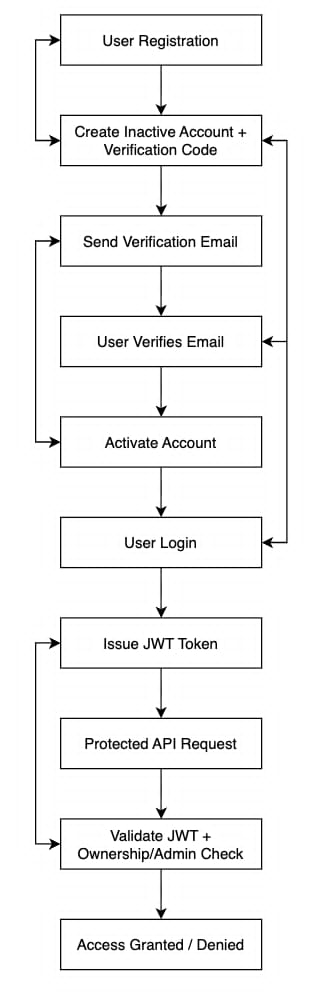
\includegraphics[width=1\linewidth,height=0.95\textheight,keepaspectratio]{images/Authentication Sequence.jpeg}
  \caption{User registration sequence diagram}
  \label{fig:seq_auth}
\end{figure}

During registration, the plaintext password is bcrypt-hashed (cost factor 12) before reaching the database. The new account is inactive until the user submits a six-digit email verification code generated by Node's \texttt{crypto} module, which expires after ten minutes.

During login, the provided password is compared against the stored hash using \texttt{bcrypt.compare()}. On success, the server signs a JWT (\texttt{userId}, \texttt{role}, \texttt{iat}, \texttt{exp}). The frontend stores this token and attaches it as an \texttt{Authorization: Bearer} header on every subsequent API request.

\textbf{Secure Password Reset Flow.}

Password resets follow a similar pattern. The server generates a 32-byte cryptographically random hex token using Node's \texttt{crypto} module, stores its bcrypt hash in the database with a one-hour expiry, and emails the plaintext token to the user. When the user submits their new password along with the token, the endpoint verifies it against the stored hash. Only after successful verification is the new password hashed and stored, and both reset token fields are cleared to prevent replay attacks.

% ─────────────────────────────────────────────────────────────────────────────
\section{Results}

\subsection{AI Pipeline Performance Results}

The pedagogical quality of AI-generated suggestions was evaluated by having the project supervisor---acting as an expert instructional design rater---blind-rate 30 randomly selected suggestions from three diverse videos. Three criteria were used:
\emph{Relevance:} Does the question test the most important concept from the preceding transcript segment, as recommended by Vural~\cite{vural2013}?
\emph{Accuracy:} Is the correct answer factually right, and are the distractors plausible but definitively incorrect?
\emph{Bloom's Alignment:} Does the AI-assigned taxonomy level match the question's actual cognitive demand, per Anderson and Krathwohl~\cite{anderson2001}?

This evaluation used English-language transcripts and outputs from the primary Groq/LLaMA pipeline. Vietnamese support was added after the study and validated only at the technical schema level, not through human pedagogical rating.

\begin{table}[H]
  \centering
  \begin{tabularx}{\linewidth}{>{\raggedright\arraybackslash}p{3.2cm} l >{\raggedright\arraybackslash}X}
    \toprule
    \textbf{Evaluation Criterion} & \textbf{Rating (E/G/P)} & \textbf{Qualitative Expert Notes} \\
    \midrule
    Pedagogical Relevance & 22/6/2 & The 2 poor suggestions were off-topic due to noisy transcript segments. \\
    \addlinespace
    Factual Accuracy & 28/2/0 & The 2 good ratings contained minor grammatical ambiguities in fill-in-the-blanks. \\
    \addlinespace
    Bloom's Taxonomy Alignment & 18/10/2 & The model struggled with high cognitive levels; ``Create'' suggestions clustered near ``Evaluate''. \\
    \bottomrule
  \end{tabularx}
  \small
  \caption{Expert AI suggestion quality ratings ($n=30$ suggestions)}
  \label{tab:ai_quality}
\end{table}

Overall, 93\% of suggestions were rated Excellent or Good on pedagogical relevance, and 100\% were rated Excellent or Good on factual accuracy. The two relevance failures both came from noisy transcript segments, consistent with the fundamental sensitivity of any transcript-based pipeline to upstream transcription quality~\cite{radford2023}.

The weakest result was Bloom's taxonomy alignment, where 12 of 30 suggestions were rated Good rather than Excellent and 2 were rated Poor. The rater noted that ``Create''-level suggestions consistently clustered near ``Evaluate'', which aligns with known limitations of general-purpose LLMs on abstract hierarchical classification tasks: models trained to predict likely continuations have no inherent understanding of Bloom's cognitive hierarchy and rely on surface-level lexical cues (e.g., ``design'', ``propose'') rather than genuine cognitive analysis. Addressing this would require either fine-tuning on annotated instructional examples or a dedicated post-generation classification step with a specialised model.

AI analysis latency was measured across 20 test runs using a standardized 5-minute technical video with 47 transcript segments.

\begin{table}[H]
  \centering
  \begin{tabularx}{\linewidth}{>{\raggedright\arraybackslash}X >{\centering\arraybackslash}p{3cm} >{\centering\arraybackslash}p{3cm}}
    \toprule
    \textbf{Performance Metric} & \textbf{Groq (LLaMA-3.3-70b)} & \textbf{Local Ollama (Llama 3.1 8B)} \\
    \midrule
    Median full generation latency (streaming)  & 8.4 seconds & 12.1 seconds \\
    \addlinespace
    Time to First Token (TTFT)  & 1.2 seconds & 2.8 seconds \\
    \addlinespace
    Median valid suggestion count & 6.4 items & 5.8 items \\
    \addlinespace
    Schema validation failure rate & 0 / 20 runs & 2 / 20 runs \\
    \bottomrule
  \end{tabularx}
    \small
  \caption{AI analysis latency and failure rates ($n=20$ runs per provider)}
  \label{tab:ai_latency}
\end{table}
\clearpage
Groq produced zero schema validation failures across all test runs. The local Ollama model produced two JSON format errors where the 8B model wrapped its response in markdown code fences (\texttt{```json}). These were caught by the \texttt{extractJsonObject()} parser and the Zod validator, preventing a frontend crash and returning a graceful error instead. The issue was fully resolved by adding an explicit instruction to the Ollama prompt: ``Return ONLY the raw JSON object. Do NOT wrap it in markdown code fences.''

The 1.2-second Time-to-First-Token with Groq is practically significant. Even though total generation takes 8.4 seconds, the instructor sees the first suggestion appear within 1.2 seconds. This makes the wait feel much shorter than the number suggests.

\textbf{Vietnamese Audio and Video Processing.}

The platform handles Vietnamese-language content at every stage of the pipeline. At the transcript acquisition stage, uploaded Vietnamese videos are transcribed by \texttt{faster-whisper}, which achieves competitive word-error rates on Vietnamese academic speech~\cite{radford2023}. YouTube-hosted Vietnamese lecture videos are processed via the automatic captions API. At the AI stage, the pipeline automatically detects Vietnamese by checking the transcript for diacritical characters (\emph{à, ă, â, đ, ơ, ư}, etc.) and switches the system prompt to Vietnamese mode. The prompt explicitly names Vietnamese topic-transition markers (``Tiếp theo'', ``Bây giờ'', ``Chuyển sang'', ``Tóm lại'') and instructs the model to return all question text, answer options, and feedback in Vietnamese while keeping JSON keys in English. The result is a fully Vietnamese-language H5P interactive video without any manual language configuration.

That said, while Vietnamese processing is functional end-to-end, its output quality falls noticeably short of the English pipeline. Two factors contribute to this gap. First, \texttt{faster-whisper}'s Vietnamese transcription is more sensitive to recording conditions: background noise, non-standard accents, and heavy domain-specific vocabulary (common in technical lectures) produce more transcription errors than equivalent English audio, which in turn degrades the quality of AI-generated questions downstream. Second, the \texttt{llama-3.3-70b-versatile} model has substantially less Vietnamese training data than English, meaning its understanding of Vietnamese sentence structure and its ability to identify appropriate topic boundaries and question-worthy content is weaker. In practice, Vietnamese-language suggestions require more instructor editing before they are ready to accept. Improving this --- through Whisper fine-tuning on Vietnamese academic speech and evaluation of Vietnamese-optimized LLM alternatives --- is a planned direction for future development.

% ─────────────────────────────────────────────────────────────────────────────
\clearpage
\subsection{API and Platform Load Performance Results}

API response times were measured with \texttt{autocannon} targeting the 12 most frequently used endpoints at 50 concurrent connections over 30 seconds.

\begin{table}[H]
  \centering
  \begin{tabularx}{\linewidth}{X >{\centering\arraybackslash}p{2.8cm} >{\centering\arraybackslash}p{2.8cm}}
    \toprule
    \textbf{Core API Endpoint} & \textbf{Median Latency (ms)} & \textbf{p99 Latency (ms)} \\
    \midrule
    \path{GET /api/videos} (Database Read)  & 12 ms  & 48 ms \\
    \addlinespace
    \path{POST /api/auth/login} (Bcrypt Hash) & 95 ms  & 180 ms \\
    \addlinespace
    \path{POST /api/videos} (FFmpeg Process)  & 220 ms & 410 ms \\
    \addlinespace
    \path{POST /api/h5p/export} (ZIP Archive) & 340 ms & 680 ms \\
    \bottomrule
  \end{tabularx}
    \small
  \caption{API endpoint response times at 50 concurrent connections}
  \label{tab:api_perf}
\end{table}

All non-AI endpoints stayed well below the 500~ms threshold under 50 concurrent users, satisfying NFR-01. The \path{POST /api/videos} endpoint is the slowest standard API call because FFmpeg thumbnail extraction runs synchronously in the request handler. Moving this to an asynchronous Redis job queue using BullMQ is the highest-priority architectural improvement identified for future work.

Ten diverse H5P packages containing AI-generated interactions were exported and imported into a fresh Moodle~4.1 test instance and a Canvas LMS sandbox. All ten packages imported without warnings or errors. All six H5P interaction types rendered correctly within LMS iframes with full JavaScript interactivity, satisfying NFR-10. This confirms the correctness of the \texttt{createH5PPackage()} implementation but does not test two-way learner data reporting, which requires xAPI integration.

% ─────────────────────────────────────────────────────────────────────────────
\subsection{Scalability Analysis}

\textbf{Tested capacity.} The platform was load-tested with \texttt{autocannon} at \textbf{50 concurrent users} making simultaneous API requests over 30 seconds. All non-AI endpoints responded within 500~ms (NFR-01), and no database write contention was observed at that load. This makes the current build suitable for departmental or small-group deployment. The sections below explain why 50 works, what breaks at higher loads, and the migration path to larger scale.

\textbf{How 50 concurrent users are handled.}
\begin{itemize}
  \item \textbf{Stateless authentication.} Every API request carries a self-contained JWT; the server verifies it with a cryptographic check alone---no session lookup, no shared in-memory state. This means any number of Node.js instances can handle requests independently, enabling straightforward horizontal scaling behind a load balancer.
  \item \textbf{SQLite read concurrency.} SQLite uses a shared-reader / exclusive-writer locking model. Read operations (fetching video lists, loading H5P content) run concurrently without blocking each other, which covers the majority of requests during browsing.
  \item \textbf{SSE streaming.} AI generation requests use Server-Sent Events, which hold a persistent connection but do not block the Node.js event loop. Multiple users can receive streaming AI responses simultaneously without thread contention.
\end{itemize}

\textbf{Bottlenecks above current scale.}
\begin{itemize}
  \item \textbf{Database writes.} SQLite serializes all writes via a single file lock. At 50 users this is rarely hit; at hundreds of simultaneous authors creating or updating content, write queuing would increase latency. A migration to PostgreSQL via the Sequelize ORM abstraction requires minimal code changes.
  \item \textbf{AI pipeline concurrency.} The Groq free-tier API allows approximately 12,000 tokens per minute, accommodating roughly 1--2 concurrent AI generation requests at full quality. Additional requests queue in the backend and are served in order. Upgrading to a paid Groq tier, or deploying a dedicated GPU inference server, removes this bottleneck for institutional deployments.
  \item \textbf{Synchronous media processing.} FFmpeg thumbnail extraction and Whisper transcription run synchronously in the Express request handler. Under concurrent video uploads this blocks the Node.js event loop and increases response times. Moving these to an asynchronous job queue (BullMQ with Redis) is the primary architectural change needed before large-scale deployment.
\end{itemize}

\subsection{Frontend Results}

Figures~\ref{fig:login_page}--\ref{fig:editor_page} show the three primary screens of the platform in light mode.

\begin{figure}[H]
  \centering
  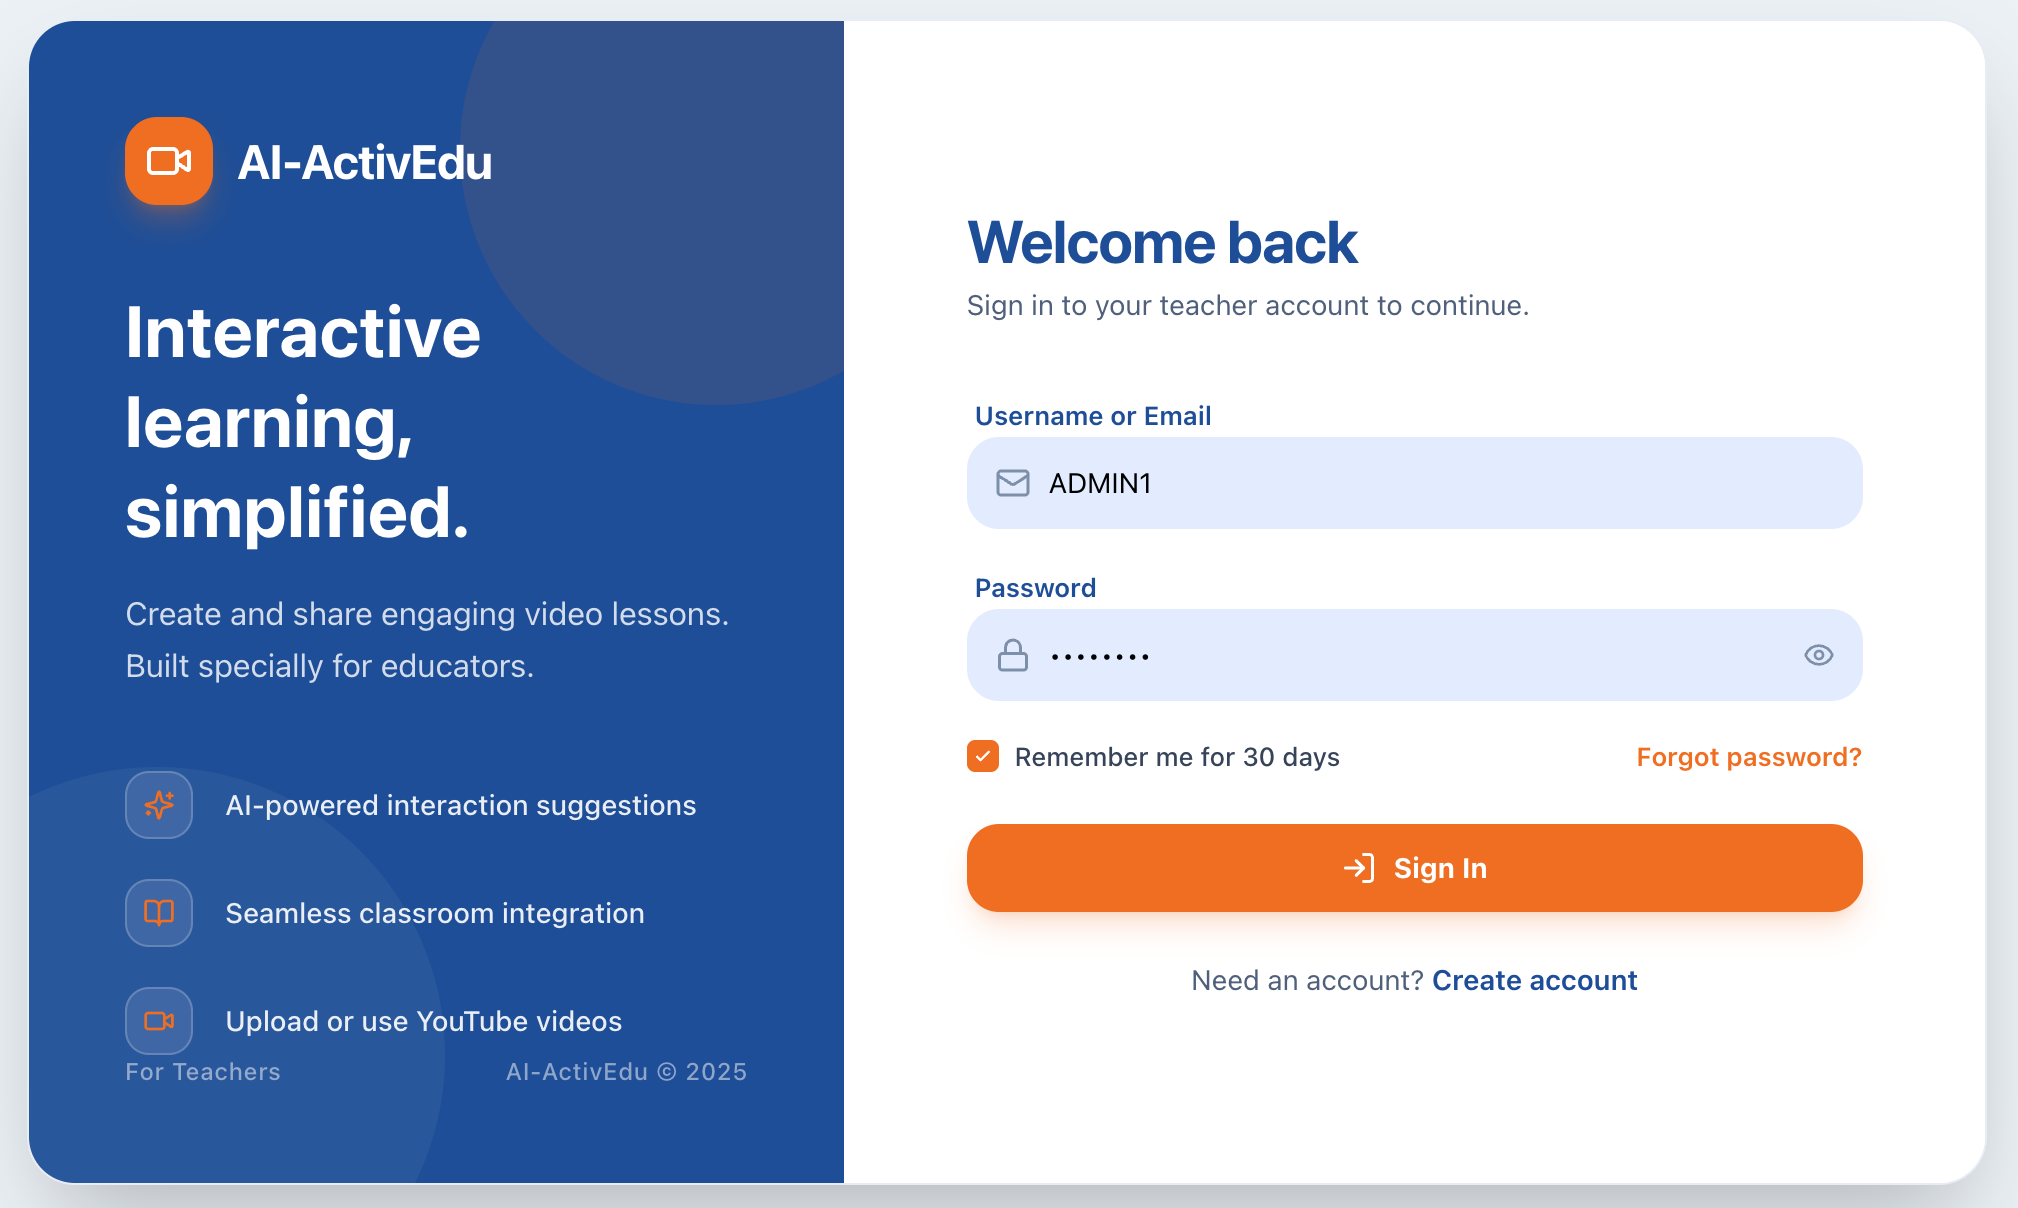
\includegraphics[width=0.9\linewidth,height=0.25\textheight]{images/login-lightmode.png}
  \caption{Login page}
  \label{fig:login_page}
\end{figure}

\begin{figure}[H]
  \centering
  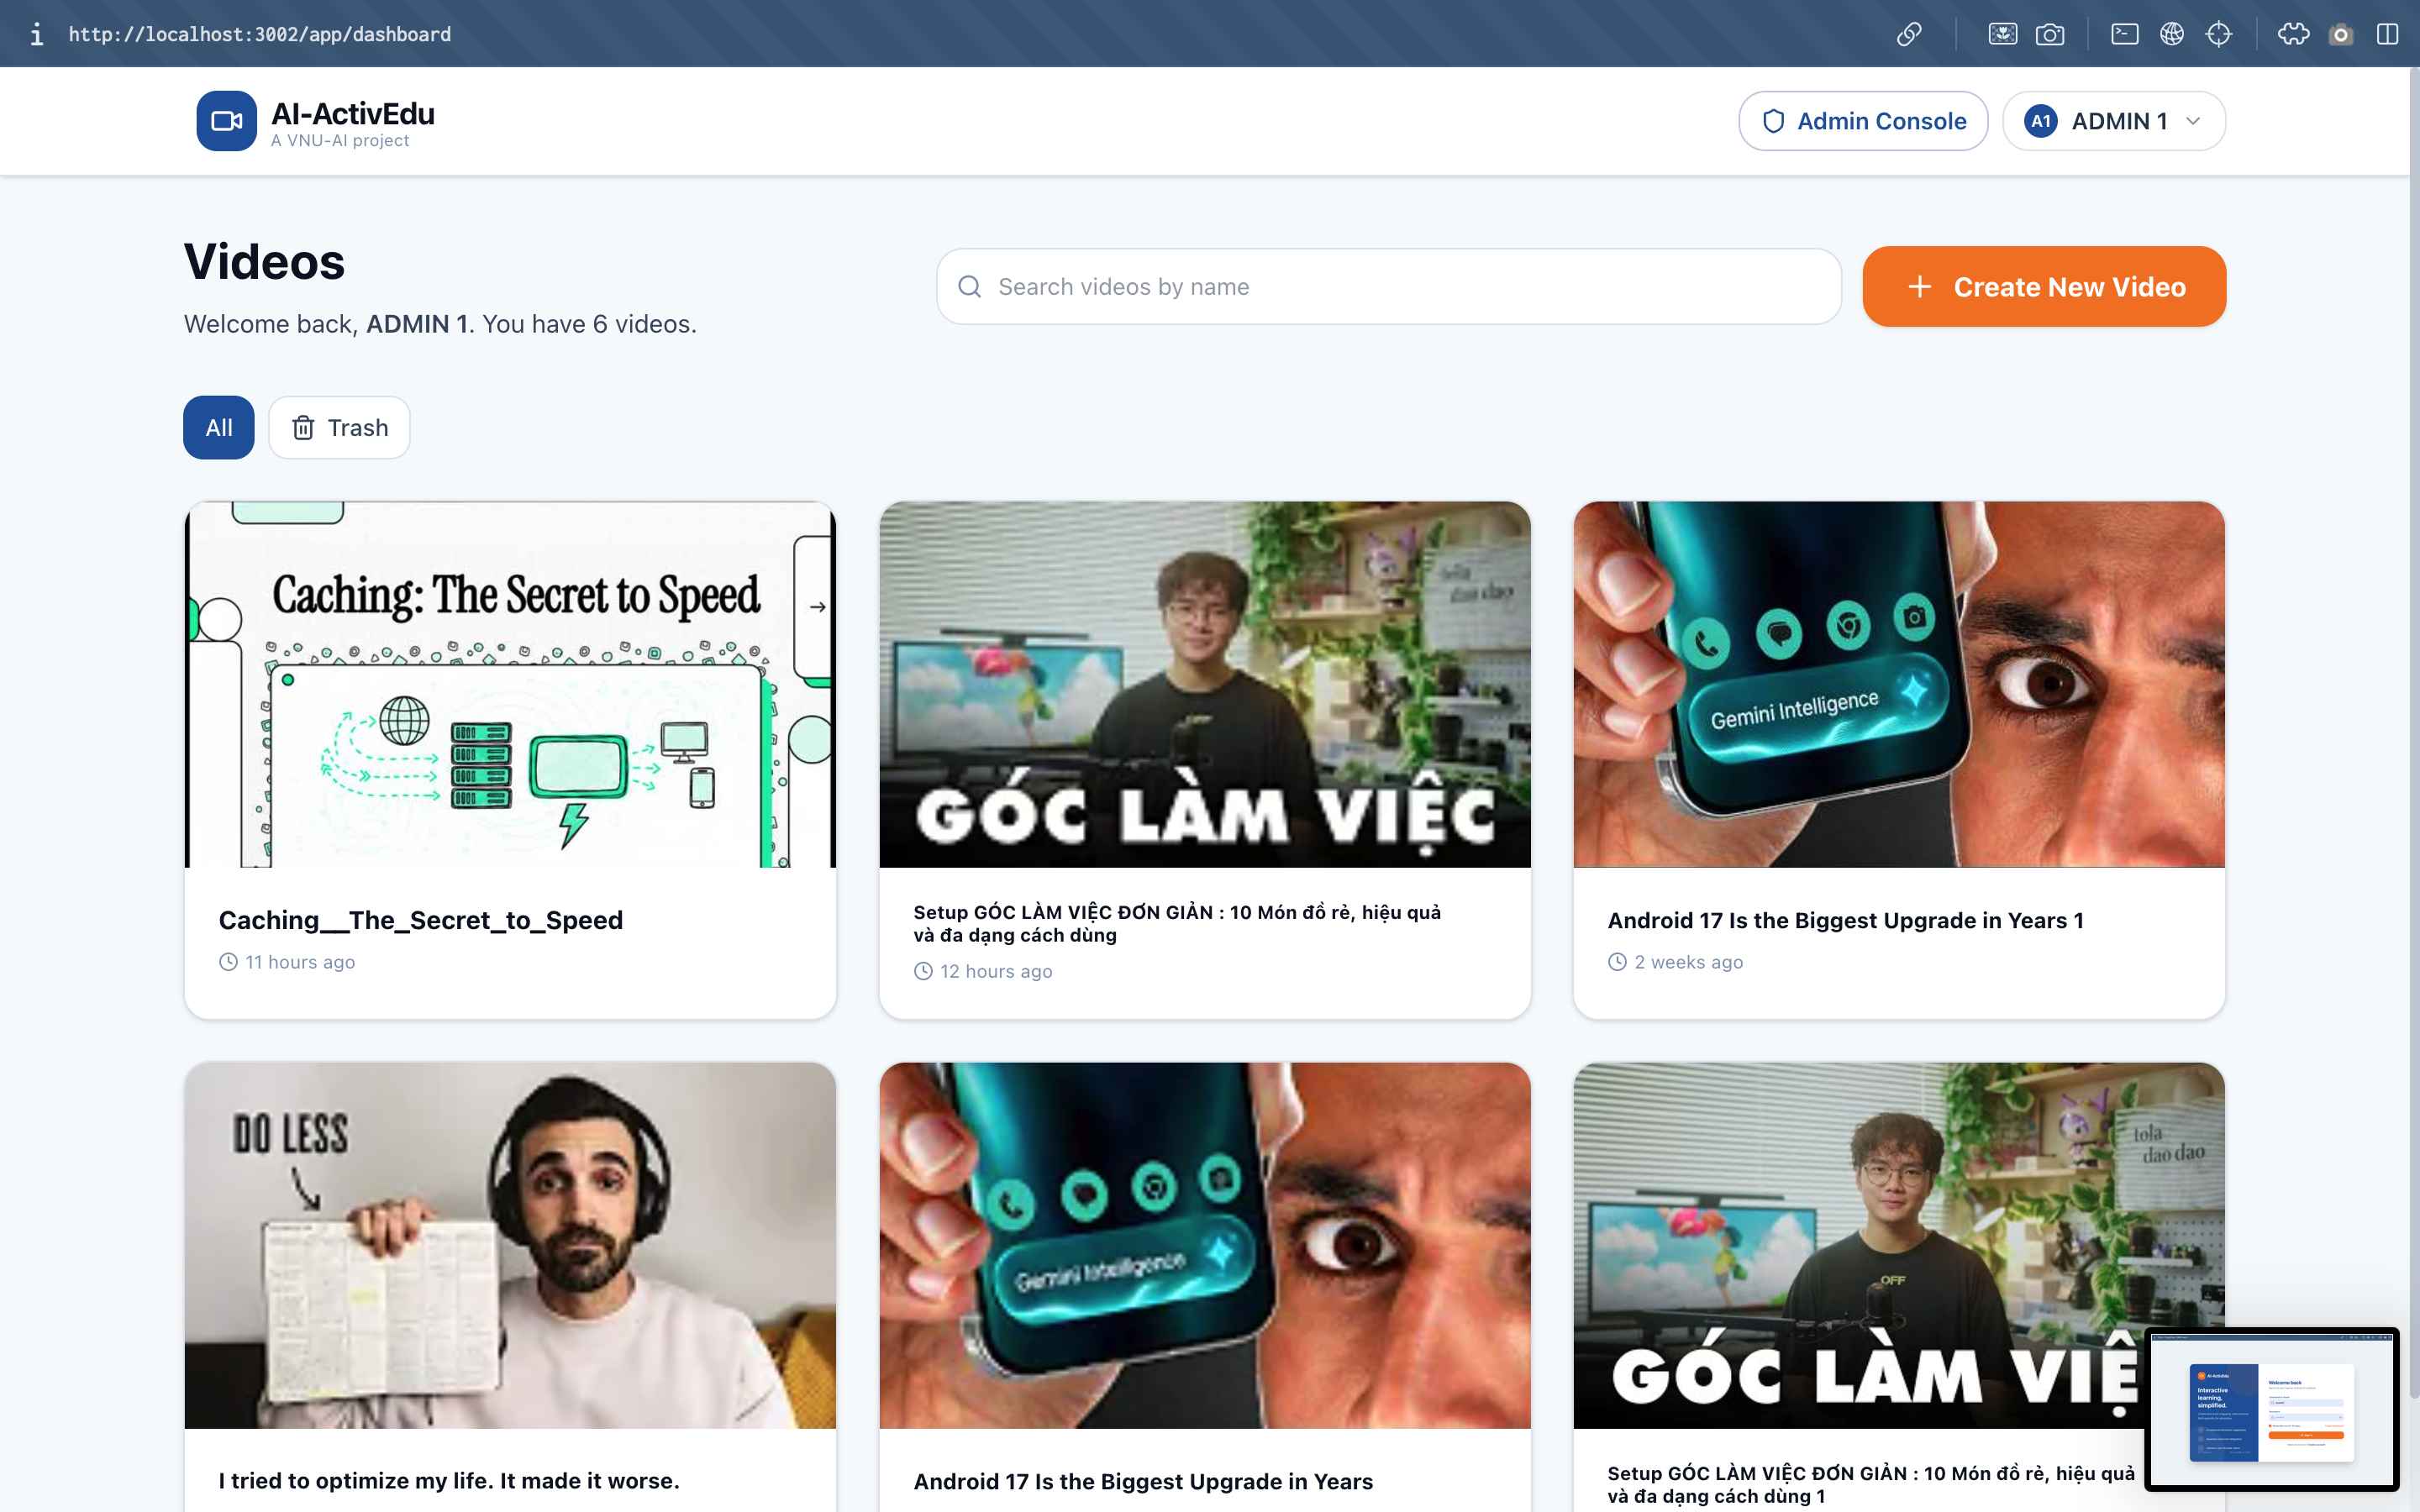
\includegraphics[width=0.9\linewidth,height=0.42\textheight,keepaspectratio]{images/home-lightmode.png}
  \caption{Dashboard (home page)}
  \label{fig:home_page}
\end{figure}

\begin{figure}[H]
  \centering
  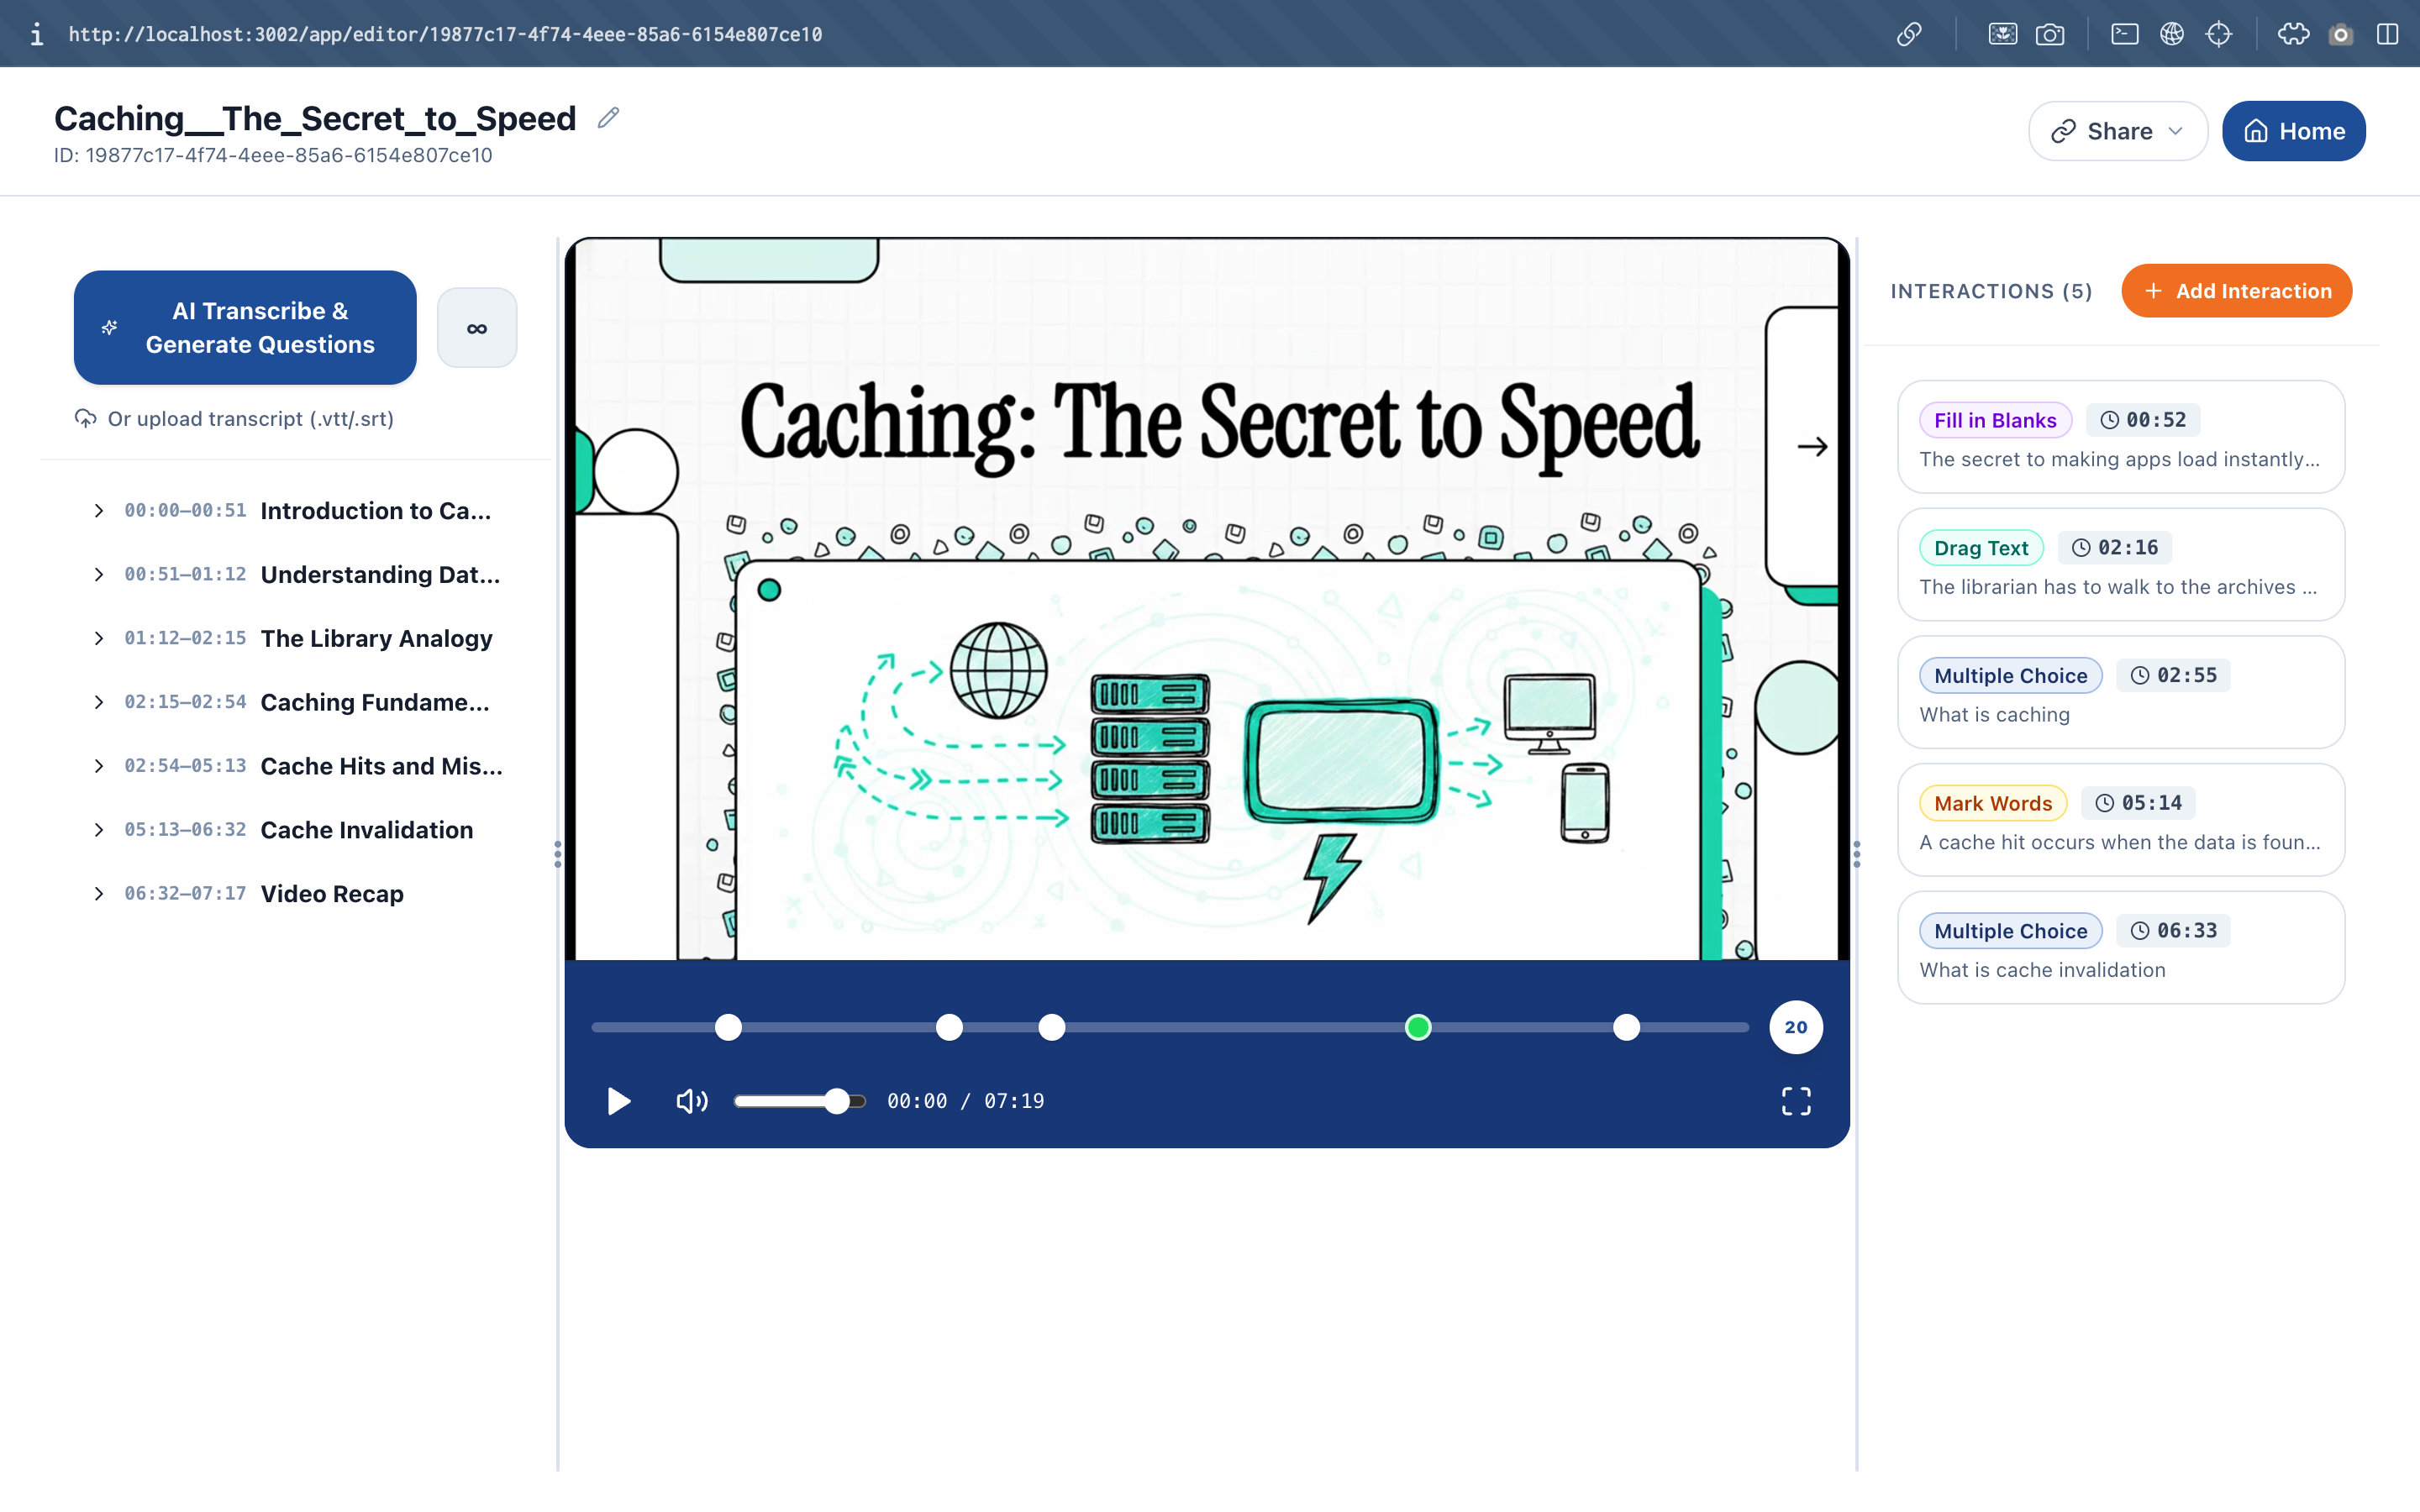
\includegraphics[width=0.9\linewidth,height=0.42\textheight,keepaspectratio]{images/editor-lightmode.png}
  \caption{Editor page}
  \label{fig:editor_page}
\end{figure}
